%\documentclass[10pt, conference, compsocconf]{IEEEtran}
\documentclass{article}\usepackage{times}
\usepackage{xcolor}
\usepackage{mathtools}
\usepackage{enumerate}
\usepackage{hyperref}
\usepackage{amssymb}
\usepackage{subfig}
\usepackage{amsmath}
\usepackage{eqnarray}
\usepackage[]{algorithm}
\usepackage{clrscode3e}
\usepackage[pdftex]{graphicx}

\DeclarePairedDelimiter{\ceil}{\lceil}{\rceil}

\begin{document}

%%%%%%%%%%%%%%%%%%%%%%%%%%%%%%%%%%%%%%%%%%%%%%%%%%%%%%%%%%%%%%%%%%%%%%%
%%%%%%%%%%%%%%%%%%%%%%%%%%%%%%%%%%%%%%%%%%%%%%%%%%%%%%%%%%%%%%%%%%%%%%%
%%
%% TITLE
%%
%%%%%%%%%%%%%%%%%%%%%%%%%%%%%%%%%%%%%%%%%%%%%%%%%%%%%%%%%%%%%%%%%%%%%%%
%%%%%%%%%%%%%%%%%%%%%%%%%%%%%%%%%%%%%%%%%%%%%%%%%%%%%%%%%%%%%%%%%%%%%%%

\title{Algorithm for watershed on graphs with plateau division by shortest path}

\author{
Aleksandar Zlateski\\ Massachusetts Institute of Technology\\ Cambridge, MA\\
{\tt\small zlateski@mit.edu}
\and
H. Sebastian Seung\\ Princeton University\\ Princeton, NJ\\
{\tt\small sseung@princeton.edu}
}



\maketitle
%\thispagestyle{empty}

%%%%%%%%%%%%%%%%%%%%%%%%%%%%%%%%%%%%%%%%%%%%%%%%%%%%%%%%%%%%%%%%%%%%%%%
%%%%%%%%%%%%%%%%%%%%%%%%%%%%%%%%%%%%%%%%%%%%%%%%%%%%%%%%%%%%%%%%%%%%%%%
%%
%% ABSTRACT
%%
%%%%%%%%%%%%%%%%%%%%%%%%%%%%%%%%%%%%%%%%%%%%%%%%%%%%%%%%%%%%%%%%%%%%%%%
%%%%%%%%%%%%%%%%%%%%%%%%%%%%%%%%%%%%%%%%%%%%%%%%%%%%%%%%%%%%%%%%%%%%%%%


\begin{abstract}
Abstract
\end{abstract}

%%%%%%%%%%%%%%%%%%%%%%%%%%%%%%%%%%%%%%%%%%%%%%%%%%%%%%%%%%%%%%%%%%%%%%%
%%%%%%%%%%%%%%%%%%%%%%%%%%%%%%%%%%%%%%%%%%%%%%%%%%%%%%%%%%%%%%%%%%%%%%%
%%
%% INTRODUCTION
%%
%%%%%%%%%%%%%%%%%%%%%%%%%%%%%%%%%%%%%%%%%%%%%%%%%%%%%%%%%%%%%%%%%%%%%%%
%%%%%%%%%%%%%%%%%%%%%%%%%%%%%%%%%%%%%%%%%%%%%%%%%%%%%%%%%%%%%%%%%%%%%%%

\section{Introduction}
The watershed transform is a standard method for image segmentation
that is based on defining a dynamical system that is discrete in space
and time.  The dynamical system steps from pixel to pixel while taking
a path of steepest descent on the pixel values.  The basins of
attraction of the dynamics constitute the resulting segmentation of
the image.

The watershed transform has previously been generalized from images to
graphs by an algorithm called ``watershed
cuts.''\cite{Cousty2009,Cousty2010}.  Here we provide a new algorithm
for watershed on graphs.  The main motivation is to handle the
division of plateaus in a systematic way. The definition of the
watershed transform becomes subtle in the presence of plateaus.  In
these ``flat'' parts of an image or graph, the direction of steepest
descent is not well-defined.  Our algorithm divides plateaus evenly,
in the sense that from any node on the plateau, the dynamics follows
the shortest path to a plateau corner.

Light and electron microscopy can now produce terascale 3D images within hours. For segmenting such large images, efficient algorithms are important. The watershed algorithm has linear runtime but tends to produce severe over-segmentation, which is typically counteracted by pre- and/or post-processing.

The Cousty algorithm alternates between depth first search (DFS) and
breadth first search (BFS) for an attractor of the gradient descent
dynamics.  It starts with DFS, switches to BFS when it enters a
plateau, and switches back to DFS when it exits a plateau, and continues alternating in this way until an attractor is found.

Our algorithm splits the search process into several passes through the graph.  The first pass explicitly computes a steepest descent graph.  The second pass removes saddle vertices and identifies plateau corners. The third pass divides plateaus via BFS. The fourth pass finds connected components.

Like watershed cuts, our algorithm has linear time complexity.
The use of multiple passes makes it possible to divide plateaus
evenly.  A second motivation for our algorithm is that it separates
the computation into two passes that are parallelizable versus two
passes that are not.  A parallel variant of our algorithm will be described in a future paper.

The input is assumed to be a disaffinity graph, in which a small edge weight indicates that the image voxels connected by the edge are likely to belong to the same segment.

The watershed transform is known to generate overly fragmented
segmentations, because every local minimum gives rise to a watershed
basin.  Therefore the image or graph is often smoothed before the
watershed transform is applied, to reduce the number of local minima.
A simple smoothing method is to set all edge weights below a threshold
$T_{\min}$ to a common low value.  

\section{The algorithm}

Consider a connected graph $G=(V,E)$ with non-negative edge
weights. An edge $\{u,v\}$ is \emph{locally maximal} for
$u$ if there is no other edge incident to $u$ with higher weight.  A
\emph{steepest ascent path} $\left\langle
v_{0},e_{0},v_{1},e_{1},v_{2}, \dots \right\rangle$ is one
for which every edge $e_{i}$ is locally minimal with respect to
$v_{i}.$

A \emph{regional minimum} $M$ is a connected subgraph of $G$ such that
there is a steepest descent path between any pair of vertices in $M$,
and every steepest descent path starting in $M$ will
stay within $M$. A vertex $v$ belongs to the \emph{basin of
  attraction} of a \emph{regional minimum $M$} if there exists a
steepest descent path from $v$ to any vertex in $M$.

In the special case where all edge weights take on unique values, the
locally minimal edge is uniquely defined for each vertex.  It follows
that the steepest descent path from every vertex is uniquely defined,
and that every vertex belongs to exactly one basin of
attraction.\footnote{Every basin consists of two vertices, and the
  steepest descent path within a basin cycles between the two
  vertices.}  The basins form a partition of the graph, which is
defined as the output of the watershed transform.

[describe standard algorithms for finding the basins.  MST, Prim, Kruskal. disjoint sets ]

More generally, a locally minimal edge for a vertex may not be unique,
because of the possibility of ties.  It follows that a steepest
descent path starting from a vertex may not be unique, and that a
vertex may belong to more than one basin of attraction.  Furthermore,
there may exist steepest descent paths that never converge to a
regional minimum but remain stuck on non-minimal ``plateaus.''  In
this case, the definition of the watershed transform is more subtle.

[describe watershed cuts]

Our algorithm explicitly computes a new directed graph $D_1$ from the
original undirected graph $G$.  The edges of $D_1$ are the steepest
descent edges of $G$, and the paths of $D_1$ are the steepest descent
paths of the original graph.  Then edges are eliminated from $D_1$ to
create $D_2$, in which all steepest descent paths (1) converge to
regional minima, (2) are unique outside regional minima, and (3)
divide plateaus evenly.

\begin{figure}
  \centering
  \subfloat[]{\protect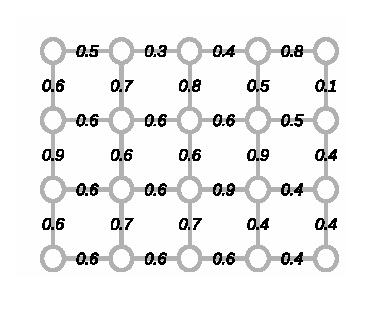
\includegraphics[scale=0.66]{fig/affinity_graph}}
  \subfloat[]{\protect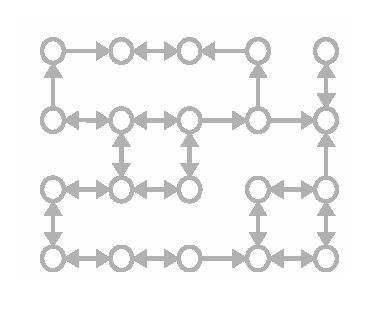
\includegraphics[scale=0.66]{fig/sd_graph}}\\
  \subfloat[]{\protect\includegraphics[scale=0.66]{fig/sd_graph_plateaus}}
  \subfloat[]{\protect\includegraphics[scale=0.66]{fig/ws_result}}

  \protect\caption{(a) A disaffinity graph; (b) derived steepest
    descent graph; (c) locally minimal plateaus (black), non-minimal
    plateau (dark gray), saddle vertex (S), plateau corners (C); (d)
    the two basins of attractions and border vertices (dark gray)}
\end{figure}

\subsection{Steepest descent graph}
The starting point is an undirected weighted graph $G$.  Replace each
edge of $G$ by edges in both directions between the same vertices
(Fig. 1(a)).  Then for every vertex retain the outgoing edge with
minimal weight and eliminate other outgoing edges.  The resulting
directed unweighted graph is called $D_1$.

If there are ties between outgoing edges (Fig. 1b), they are resolved
by assuming a pre-existing ordering of the vertices.  The ordering
could be represented by a bijective map
$\alpha:V\to\{1,2,...,|V|\}$. We refer to $\alpha(u)$ as the index of
$u$ (Fig. 2a).  The winning edge is the one pointing to the vertex
with the lowest index.

If a pair of vertices has edges in both directions, they are
represented by a single ``bidirectional edge'' in Fig. 1b, and we will
use this term for convenience.  Threrefore, the edges of any vertex in
$D_1$ can be classified as incoming, outgoing, and bidirectional.

A directed path in $D_1$ is a path of steepest descent in $G$.  A
steepest ascent graph can be defined analogously using edges of
maximal weight. Either steepest ascent or descent can be used without
loss of generality.

\begin{figure}
  \centering
  \subfloat[]{\protect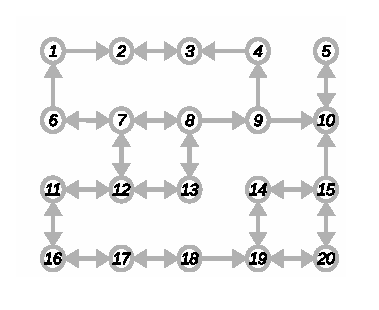
\includegraphics[scale=0.66]{fig/sd_graph_ordered}}
  \subfloat[]{\protect\includegraphics[scale=0.66]{fig/sd_graph_plateaus_ordered}}\\
  \subfloat[]{\protect\includegraphics[scale=0.66]{fig/sd_graph_plateaus_modified}}
  \subfloat[]{\protect\includegraphics[scale=0.66]{fig/final_segmentation}}

  \protect\caption{(a) Vertex indices; (b) distances to the nearest
    plateau corner; (c) modifications to the steepest descent graph;
    (d) final watershed partition of the graph}
\end{figure}

\subsection{Plateau division}
While no vertex in $D_1$ has two or more outgoing edges, directed
paths are still not uniquely defined, because of the existence of
plateaus.

A \emph{plateau} is a connected component of the subgraph of $D_1$
containing only bidirectional edges.  A plateau \emph{corner} is a
plateau vertex with an outgoing edge.
% there can't be more than one, since saddles were eliminated, right?
\emph{Locally minimal} plateaus contain no corners; they are
equivalent to the regional minima of the original graph.  If a
directed path of $D_1$ enters a locally minimal plateau, it remains
within the plateau for all future time.

\emph{Non-minimal} plateaus contain one or more corners.  If a
directed path enters a non-minimal plateau, it may stay within the
plateau, or exit through one of the corners.  These types
of plateaus are illustrated in Fig. 1c.

We would like to alter $D_1$ so that any directed path that enters a
non-minimal plateau will not get stuck there, but will eventually
exit.  This guarantees that any directed path will eventually reach a
locally minimal plateaus, i.e., locally minimal plateaus are the only
attractors of the dynamics.

Furthermore, we would like a non-minimal plateau with multiple corners
to be divided evenly, in the following sense.  From each vertex in the
plateau, the directed path should lead to the nearest corner, where
nearest is defined based on graph distance.  If there is a tie between
corners, it should be resolved using the same ordering function as before. 

Both of these goals are achieved by applying the following algorithm
to every non-minimal plateau.  We initialize a global FIFO queue $Q$,
mark all the corner vertices as visited and insert them into $Q$ in
increasing order of their index. While $Q$ is not empty we remove the
vertex $v$ from the front of the queue, and loop over all its
bidirectional edges $\{v,u\}$.  If $u$ has not yet been visited, we
mark it as visited, insert it to the back of the queue, and change the
edge from bidirectional to incoming $(v\leftarrow u)$. If $u$ has
already been visited, we remove the bidirectional edge $\{v,u\}$
completely.

After this BFS is completed, the non-minimal plateau will no longer
have bidirectional edges, and every vertex will have a single outgoing
edge.  Furthermore, every directed path will lead to the nearest
corner.

\subsection{Connected components}
After applying this BFS to every non-minimal plateau, we arrive at the
modified steepest descent graph $D_2$ (Fig. 2c).  Every directed path eventually reaches a locally minimal plateau.  The path from any vertex to its corresponding locally minimal plateau is unique.  Therefore, the graph can be segmented into the basins of attraction of the dynamics.

The basins can be found by regarding $D_2$ as an undirected graph and
computing its connected components.  [via what algorithm]

\section{Formal description}
Our algorithm runs in linear time with respect to the number of edges
in $G$ and produces an optimal partitioning as defined
in~\cite{Cousty2009}. The total number of segments in the partitioning
will equal to the total number of \emph{regional minima}.

%We defer the detailed algorithm listing, the proof of correctness and running time analysis to the supplementary material.

\begin{enumerate}
\item Apply the threshold $T_{\min}$ and $T_{\max}$:
  \begin{enumerate}
  \item Remove each $\{u,v\}$ from $E$ if $w(\{v_i,u\}) > T_{\max}$.
  \item For each $\{u,v\}$ from $E$ set $w(\{v_i,u\}) = 0$ if
    $w(\{v_i,u\}) < T_{\min}$.
  \item Remove singleton vertices (vertices with no incident edges in
    $E$). Mark them as background.
  \end{enumerate}
\item Create $G'$. Set $V'=V$ and $E'=\emptyset$. For each vertex $v_i
  \in V'$:
  \begin{enumerate}
  \item Calculate $M_i = \min_{u \in V', \{v_i,u\} \in
    E}\{w(\{v_i,u\})\}$.
  \item For each $u \in V'$ such that $\{v_i,u\} \in E$ add $(v_i,u)$
    to $E'$ if $w(\{v_i,u\})=M_i$.
  \end{enumerate}
\item Modify $G'$ to remove all saddle vertices. For each vertex $v
  \in V$ that has more than one outgoing edge, keep only one outgoing
  edge pointing to a vertex with the minimal index.
\item Modify $G'$ to split the non-minimal plateaus:
  \begin{enumerate}
  \item Initialize a FIFO queue $Q$.
  \item For each vertex $v \in V'$, check whether the vertex has at
    least one outgoing edge and one bidirectional edge (check whether
    the vertex is a plateau corner). If it does mark it as visited and
    add it to the end of $Q$.
  \item While $Q \neq \emptyset$, let $u$ be the first element of $Q$
    and remove it from $Q$. For all $v$ such that $(u,v) \in E'$ and
    $(v,u) \in E'$ remove $(u,v)$ from $E'$. If $v$ is visited remove
    $(v,u)$ from $E'$ as well, otherwise mark $v$ as visited and add
    it to the end of $Q$.
  \end{enumerate}
\item Replace all unidirectional edges with bidirectional edges. For
  each $(u,v) \in E'$ add $(v,u)$ to $E'$ if not already there.
\item Return connected components of the modified $G'$.
\end{enumerate}

In the first step of the algorithm we apply the thresholds and mark
the singleton vertices as background, as desired by the output. We
expect all the other vertices to be assigned to a watershed basin. In
the second step we create the steepest descent graph. In the steps 3
we make sure that all the saddle vertices are removed. After this step
there will be no vertices with more than one outgoing edge. The step 4
splits the plateaus. In the breadth first search, while examining the
plateau vertices, we make sure that all the vertices have only one
outgoing edge. The breadth first search order will ensure that we keep
the edge on the path to the closest plateau corner (with the minimal
index). After the step 4 all vertices that don't belong to a regional
minima will have a single outgoing edge, hence there will be an unique
steepest descent path to a single regional minima. Therefore, all the
vertices will be uniquely assigned to a basin. The step 5 just makes
sure there's also a path from a regional minima to all vertices in its
basin of attraction so that we can just apply connected components in
order to obtain the watershed basins.

As we operate on a connected graph we assume $O(|E|) \ge O(|V|)$. The
first three steps of the algorithm visit each edge constant number of
times. In the step 4, we visit each vertex at most once. While
visiting each vertex we visit edges incident to it constant number of
times. The step 5 also visits each edge at most once. As the
complexity of connected components is $O(|E|)$, we get our overall
complexity to be $O(|E|)$.

\section{Reducing over-segmentation}.

 Noisy values of \emph{disaffinities} can produce severe
 over-segmentation (Fig. 3(c)). In order to reduce the
 over-segmentation we often merge adjacent segments with the
 \emph{saliency} below some given threshold
 $T_{\min}$~\cite{Najman1996}. The \emph{saliency} of two adjacent
 segments is defined as the value of the minimal \emph{disaffinity}
 between the vertices of the two segments. That means that we are
 confident that \emph{disaffinities} below $T_{\min}$ connect vertices
 of the same segment. An equivalent segmentation can be obtained by
 replacing the weights of all edges in $G$ with the weight smaller
 than $T_{\min}$ to a common low value (e.g. $0$) before applying the
 watershed transform. We prove this claim in the supplementary
 material. To show confidence about high values of
 \emph{disaffinities}, and in order to prevent undesired mergers, we
 introduce a threshold $T_{\max}$ by erasing all the edges from $G$
 with the weight higher than $T_{\max}$, and essentially setting them
 to $\infty$. The $T_{\max}$ threshold can produce singleton vertices
 in $G$. The singleton vertices are not assigned to any \emph{basin of
   attraction} and are considered background, which is often a desired
 result.

\begin{enumerate}
\item Applying watershed transform and then merging all basins with
  saliency smaller than $T_{\min}$, and
\item Applying watershed on a graph where with all the edges with
  weight smaller than $T_{\min}$ are replaced with edges with weight
  of $0$
\end{enumerate}
are equivalent. We first prove the following lemma:

\subsubsection{Lemma 1}
\emph{Examine a watershed transform $W$ of $G$ and watershed transform
  $W'$ obtained by applying a threshold $T_{\min}$ on $G$. Let
  $\{B_1,B_2,\dots\}$ be the watershed basins of $W$ and
  $\{B'_1,B'_2,\dots\}$ the watershed basins of $W'$. For each $B_i$
  there exist $B'_j$ such that $B_i \subseteq B'_j$}.


\subsubsection{Proof}.
The steepest descent graph containing only vertices in $V$ that are
not incident to any edge with the weight smaller than $T_{\min}$ will
stay unmodified, even after splitting the plateaus and getting rid of
the saddle vertices. All other vertices will became a part of a
regional minima (locally minimal plateau in the steepest descent
graph). All previous locally minimal edges will stay locally
minimal. Therefore applying the threshold $T_{\min}$ just introduces
bidirectional edges to the steepest descent graph. Therefore, a
connected component in the modified steepest descent graph of $G$ has
to be a subset of a connected component of the modified steepest
descent graph of $G$ after applying $T_{\min}$.

Watershed basins of $W'$ are connected. Hence, they can be obtained by
merging watershed basins of $W$. We prove that the result of 1. and
2. are equivalent by showing that two neighboring basins of $W$, $B_i$
and $B_j$ will be merged in 1. if and only if they are merged in 2.

Let's examine two watershed basins of $W$, $B_i$ and $B_j$. If there
is an edge $\{u,v\}$ in $G$ such that $u \in B_i$ and $v \in B_j$ with
the weight smaller than $T_{\min}$, then $u$ and $v$ will be part of
the same regional minima in $W'$. Hence, the two basins of $W$ belong
to a single basin of $W'$. We also know that the saliency between
$B_i$ and $B_j$ has to be smaller than $T_{\min}$, therefore they will
belong to the same segment when applying the algorithm 1. Similarly,
if the saliency $d_{ij}$ between $B_i$ and $B_j$ is below $T_{\min}$,
then there exist an edge $\{u,v\}$ in $G$ such that $u \in B_i$ and $v
\in B_j$ with the weight equal to $d_{ij} < T_{\min}$. Therefore $u$
and $v$ will be part of the same regional minima, and $B_i$ and $B_j$
will be part of the same watershed basin in $W'$.

%%%%%%%%%%%%%%%%%%%%%%%%%%%%%%%%%%%%%%%%%%%%%%%%%%%%%%%%%%%%%%%%%%%%%%%
%%%%%%%%%%%%%%%%%%%%%%%%%%%%%%%%%%%%%%%%%%%%%%%%%%%%%%%%%%%%%%%%%%%%%%%
%%
%% REFERENCES
%%
%%%%%%%%%%%%%%%%%%%%%%%%%%%%%%%%%%%%%%%%%%%%%%%%%%%%%%%%%%%%%%%%%%%%%%%
%%%%%%%%%%%%%%%%%%%%%%%%%%%%%%%%%%%%%%%%%%%%%%%%%%%%%%%%%%%%%%%%%%%%%%%


{\small
\bibliographystyle{ieeetr}
\bibliography{./ref/bib}
}

\end{document}

\subsection{Assigning border vertices}
In Fig. 1(d) we show the \emph{basins of attraction} of the two
\emph{regional minima}. The \emph{border} vertices are shown in dark
gray and belong to both \emph{basins of attraction}. Watershed
cuts~\cite{Cousty2009,Cousty2010} assign \emph{border} vertices with a
single constraint that all the \emph{basins of attraction} have to be
connected.

